\chapter{Teoria}
\label{c3}

\section{Wstęp}
\label{c31}

W danym rozdziale zostanie zawarty opis architektury oraz główne komponenty wykorzystywane przez App Inventora. Pomoże to zrozumieć zalety oraz wady powyższego narzędzia.

\section{Architektura}
\label{c32}

Każda aplikacja ma swoją wewnętrzną strukturę, którą trzeba dokładnie zrozumieć, aby tworzyć efektywne oprogramowanie. Architektura aplikacji składa się głównie z 2 części: komponenty oraz ich zachowanie. Można z pewnym dystansem przyjąć że za komponenty odpowiada widok Designera, a za zachowanie komponentów widok edytora.

\begin{figure}[th] 
\centering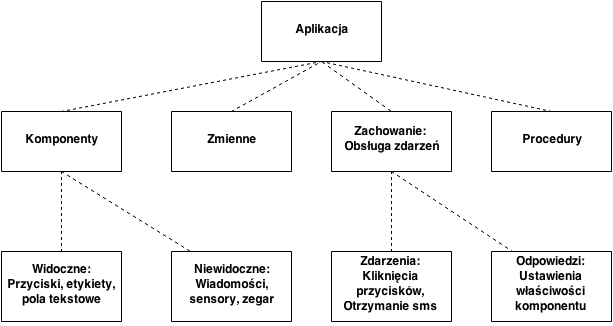
\includegraphics[width=10cm]{figures/architektura}
\caption{Architektura aplikacji stworzonej przez App Inventora\cite{appinventor:architektura}}
\end{figure}

\subsection{Komponenty}
\label{c321}

Komponenty można podzielić na 2 rodzaje: widoczne oraz niewidoczne. 
\begin{itemize}
\item Widoczne są to takie, które użytkownik widzi gołym okiem np. przyciski, etykiety, pola tekstowe. Definiują one interfejs użytkownika.
\item Niewidocznych komponentów, jak sama nazwa wskazuje, użytkownik nie widzi. Nie są one częścią interfejsu. Dostarczają one dostępu do wbudowanych funkcjonalności telefonu. Są to różne sensory np. akcelerometr, moduł gps, komponent zamiany tekstu na mowę itp.
\end{itemize}

Oba rodzaje komponentów posiadają zbiór swoich właściwości. Właściwości danego komponentu są to informacje jakie komponent posiada. Etykieta posiada między innymi rodzaj, wielkość, dekorację, kolor czcionki, wielkość, widoczność etykiety. Użytkownik nie widzi danych właściwości, obserwuje on rezultat konkretnych ustawień na ekranie urządzenia.

\subsection{Zachowanie aplikacji}
\label{c322}
Zrozumienie zasady tworzenia komponentów i ich właściwości jest proste. Nazwy komponentów są intuicyjne, więc nie powinno być problemu z odnalezieniem tego, który interesuje programistę. Z drugiej strony zachowanie komponentów może okazać się bardziej skomplikowane. Mimo wszystko App Inventor stara się wizualizować bloki opisujące zachowanie w jak najprostszej formie.

Kiedy zaczynano pisać aplikacje, można było je porównać do recept, gdzie ciąg zdarzeń ukazany jest jako liniowa sekwencja instrukcji. Typowa aplikacja może uruchomić transakcję w banku, dokonać pewnych obliczeń, zmodyfikować stan konta i na koniec wyświetlić nowe saldo.\cite{appinventor:architektura}

W dzisiejszych czasach większość aplikacji nie wpasowuje się w powyższy schemat. Zamiast wykonywać ciąg instrukcji w odpowiedniej kolejności, reagują na zdarzenia, które są inicjowane przez użytkownika danej aplikacji. Jednym z przykładów jest kliknięcie przycisku lub trzęsienie telefonem, który jest zaprogramowany tak, aby na każdy bodziec móc umieć odpowiedzieć. Wiele zdarzeń jest inicjowanych przez użytkownika, ale są też wyjątki. Aplikacja może reagować na zdarzenia, które w nie wymagają interakcji z użytkownikiem. Często są to niewidoczne komponenty umieszczone w Designerze. Poniższy rysunek prezentuje aplikację otoczoną wieloma zdarzeniami.

\begin{figure}[th] 
\centering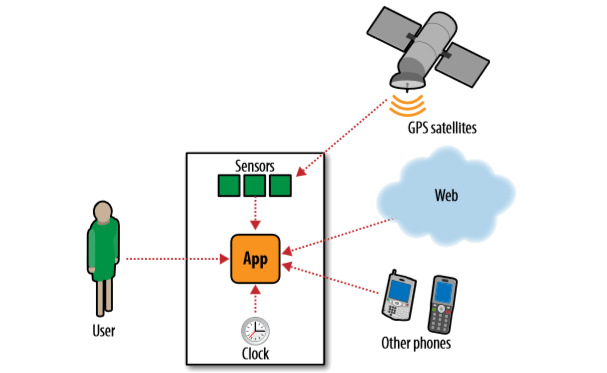
\includegraphics[width=10cm]{figures/events}
\caption{Aplikacja reagująca na zdarzenia zewnętrzne i wewnętrzne\cite{appinventor:architektura}}
\end{figure}

Jednym z powodów dlaczego App Inventor jest tak intuicyjny jest zastosowaniej prostej koncepcji nazywania zdarzeń. Zdefiniowanie zdarzenia polega na przeciągnięciu go z palety na główny ekran, a następnie napisanie konkretnego zachowania. Przykładem takiego zdarzenia jest obsługa akcelerometru. Po zatrzęsieniu telefonem, pojawia się tekst "Shaking!".

\begin{figure}[th] 
\centering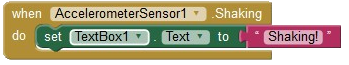
\includegraphics[width=10cm]{figures/shakingEvent}
\caption{Obsługa zdarzenia trzęsienia telefonem}
\end{figure}

Zdarzenia można podzielić w zależności od jego typu:
\begin{itemize}
\item Zainicjowane przez użytkownika - najbardziej popularny typ zdrzania - głównie jest to obsługa zdarzeń dotyku ekranu.
\item Inicjalizujące - są wykonywane, gdy dany komponent jest tworzony.
\item Czasowe - są uruchamiane, co pewien interwał czasowy.
\item Animacje - są zależne od obiektów (spritów) które zostały stworzone. Mogą zostać uruchomione gdy obiekty ze sobą kolidują, wylatują poza ekran.
\item Zewnętrzne - są uruchamiane gdy urządzenie odbierze jakiś sygnał zewnętrzny typu, odczyt pozycji urządzenia z satelity, reakcja na przychodzący sms.
\end{itemize}

Programowanie aplikacji odbywa się poprzez zdefiniowanie interfejsu, a następnie napisanie zachowania danej aplikacji, dla różnych zdarzeń, które mogą wystąpić. Inaczej mówiąc, tworzymy najpierw komponenty w Designerze i ustawiamy im właściwości. Kiedy otrzymaliśmy interesujący nas wygląd zabieramy się za opisanie zdarzeń.

\section{Debugowanie aplikacji}
\label{c33}

Najłatwiejszy sposób instalacji i testowania aplikacji odbywa się przez wifi. Musimy pobrać dodatkową aplikację na urządzenie z systemem android. Następnie na stronie app inventora uruchamiamy opcję połączenia z telefonem i pojawia nam się na monitorze kod QR, który skanujemy telefonem, z pomocą ściągniętej aplikacji. Po tych czynnościach aplikacja zostaje automatycznie zainstalowana na telefonie. Aplikacja dodatkowo automatycznie uaktualnia wprowadzone zmiany, nie trzeba jej uruchamiać ponownie. Jest to rekomendowany sposób, jednak istnieją jeszcze 2 dodatkowe. Jeżeli nie posiadamy urządzenia z systemem Android możemy użyć emulatora. Trzecia opcja to możemy połączyć telefon z komputerem i aplikacją przez kabel USB.